\documentclass[a4paper,12pt]{article}

% Math packages
\usepackage{amsmath, amssymb, amsthm}
\usepackage{tikz}
\usepackage{subcaption}

% Header
\usepackage{fancyhdr}
\pagestyle{fancy}

\fancyhead{} % clear default
\fancyhead[L]{Anton Thestrup Jørgensen}
\fancyhead[R]{s194268}

\begin{document}

\section*{Question 1}

\subsection*{a)}

First we see that $\psi(0) = 0$. Now let $z_1=a+ib$ and $z_2=c+id$. Then
\[
z_1+z_2=(a+c)+i(b+d),
\]
so
\[
\psi(z_1+z_2)= (a+c)+(b+d) \pmod 2.
\]
On the other hand,
\[
\psi(z_1)+\psi(z_2) = (a+b)+(c+d) \pmod 2.
\]

By associativity and commutativity of addition modulo 2, these expressions are equal, hence $\psi$ preserves addition. It follows from the two facts above, that $\psi$ is a group homomorphism.

We also have $\psi(1)=1$, so the multiplicative identity is preserved. For multiplication, we have
\[
z_1 z_2 = (ac - bd) + i(ad + bc).
\]
Applying $\psi$ gives
\[
\psi(z_1 z_2) = (ac - bd) + (ad + bc) \pmod 2
= ac + bd + ad + bc \pmod 2.
\]
Meanwhile,
\[
\psi(z_1)\psi(z_2) = (a+b)(c+d) \pmod 2
= ac + ad + bc + bd \pmod 2.
\]
By commutativity of addition modulo 2, these expressions are equal. Thus $\psi$ preserves multiplication. 



Therefore $\psi$ is a ring homomorphism.

\subsection*{b)}
The kernel of $\psi$ is given by
\[
\mathrm{ker}(\psi) = \{ z = a+ib \in \mathbb{Z}[i] \mid a + b = 0 \pmod{2} \}.
\]
That is, every gaussian integer where the sum of the real and imaginary parts is even. See Figure \ref{fig:gaussian_integers}.


\begin{figure}[h]
    \centering
    % TikZ picture goes here

    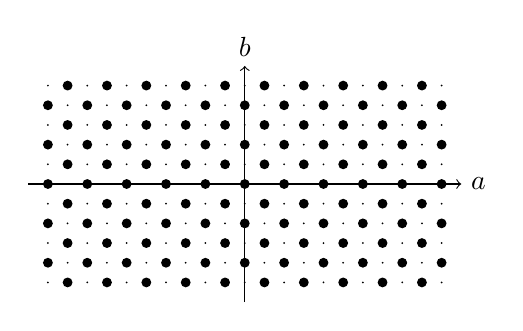
\begin{tikzpicture}[scale=0.25]

    % Axes
    \draw[->] (-11,0) -- (11,0) node[right] {$a$};
    \draw[->] (0,-6) -- (0,6) node[above] {$b$};

    % Gaussian integer points
    \foreach \a in {-10,-9,...,10} {
    \foreach \b in {-5,-4,...,5} {
        \pgfmathtruncatemacro{\s}{mod(\a+\b,2)}
        % s = 0 means even, 1 means odd
        \ifnum\s=0
        \fill (\a,\b) circle (0.25); % even: larger
        \else
        \fill (\a,\b) circle (0.05); % odd: smaller
        \fi
    }
    }

    \end{tikzpicture}

    \caption{$\mathbb{Z}[i]$. Larger dots represent elements in the kernel of $\psi$.}
    \label{fig:gaussian_integers}
\end{figure}


\subsection*{c)}

To use the ring isomorphism theorem, we must first show that $\langle 1 + i\rangle $ is equal to the kernel of $\psi$.

First we show that $\langle 1 + i\rangle $ is contained in the kernel of $\psi$. Take any $z \in \langle 1 + i\rangle $. By definition of ideals, there exists a $k \in \mathbb{Z}[i]$ such that
\[z = (1 + i) \cdot k.
\]
Let $k = m + in$, where $m, n \in \mathbb{Z}$. Then
\[z = (1 + i)(m + in) = (m - n) + i(m + n).
\]
Applying $\psi$ gives
\[\psi(z) = (m - n) + (m + n) \pmod{2} = 2m \pmod{2} = 0.
\]
Therefore $z \in \mathrm{ker}(\psi)$, and since $z$ was arbitrary, we have shown that $\langle 1 + i\rangle  \subseteq \mathrm{ker(\psi)}$.

Now we show that $\mathrm{ker}(\psi)$ is contained in $\langle 1 + i\rangle $. Take any $z \in \mathrm{ker}(\psi)$. Let $z = a + ib$, where $a, b \in \mathbb{Z}$. Then, by definition of the kernel, we have
\[\psi(z) = a + b \pmod{2} = 0,
\]
so $a + b$ is even. This means that either both $a$ and $b$ are even, or both are odd.

Now divide $a + ib$ by $1 + i$:
\[
\frac{a + ib}{1 + i} = \frac{(a + ib)(1 - i)}{(1 + i)(1 - i)} = \frac{(a + b) + i(b - a)}{2} = \frac{a + b}{2} + i\frac{b - a}{2}.
\]

Since $a$ and $b$ are both even or both odd, both $\frac{a + b}{2}$ and $\frac{b - a}{2}$ are integers. Therefore, $\frac{a + ib}{1 + i} \in \mathbb{Z}[i]$, so $z = a + ib$ is a multiple of $1 + i$ in $\mathbb{Z}[i]$. Thus, $z \in \langle 1 + i\rangle $, and since $z$ was arbitrary, we have shown that $\mathrm{ker}(\psi) \subseteq \langle 1 + i\rangle $.

Combining the two inclusions, we have shown that $\mathrm{ker}(\psi) = \langle 1 + i\rangle $. We can now use the ring isomorphism theorem, since we have established that $\psi$ is a ring homomorphism from $\mathbb{Z}[i]$ to $\mathbb{Z}_2$ with kernel $\langle 1 + i\rangle $ and image $\mathbb{Z}_2$, to conclude that
\[\mathbb{Z}[i] / \langle 1 + i\rangle  \simeq \mathbb{Z}_2.
\]

\subsection*{d)}

\begin{figure}[h]
\centering

% ------------------- Multiples of 2 -------------------
\begin{subfigure}{0.25\textwidth}
\centering
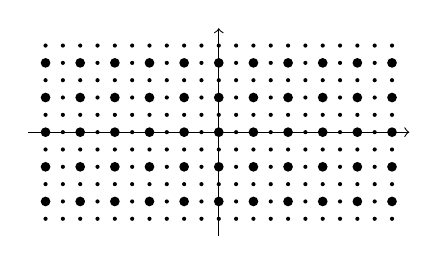
\begin{tikzpicture}[scale=0.22]

\draw[->] (-11,0) -- (11,0);
\draw[->] (0,-6) -- (0,6);

\foreach \a in {-10,-9,...,10} {
  \foreach \b in {-5,-4,...,5} {
    \pgfmathtruncatemacro{\highlight}{(mod(\a,2)==0 && mod(\b,2)==0 ? 1 : 0)}
    \ifnum\highlight=1
      \fill (\a,\b) circle (0.28);
    \else
      \fill (\a,\b) circle (0.12);
    \fi
  }
}

\end{tikzpicture}
\end{subfigure}
\hfill
% ------------------- Multiples of 3 -------------------
\begin{subfigure}{0.25\textwidth}
\centering
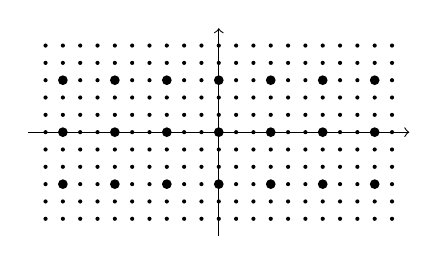
\begin{tikzpicture}[scale=0.22]

\draw[->] (-11,0) -- (11,0);
\draw[->] (0,-6) -- (0,6);

\foreach \a in {-10,-9,...,10} {
  \foreach \b in {-5,-4,...,5} {
    \pgfmathtruncatemacro{\highlight}{mod(\a*\a + \b*\b, 3)==0 ? 1 : 0}
    \ifnum\highlight=1
      \fill (\a,\b) circle (0.28);
    \else
      \fill (\a,\b) circle (0.12);
    \fi
  }
}

\end{tikzpicture}
\end{subfigure}
\hfill
% ------------------- Multiples of 4 -------------------
\begin{subfigure}{0.25\textwidth}
\centering
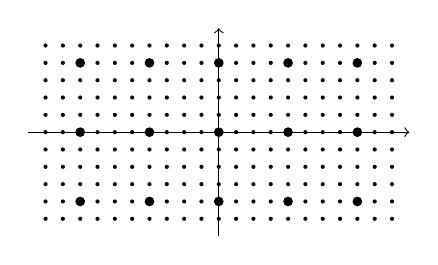
\begin{tikzpicture}[scale=0.22]

\draw[->] (-11,0) -- (11,0);
\draw[->] (0,-6) -- (0,6);

\foreach \a in {-10,-9,...,10} {
  \foreach \b in {-5,-4,...,5} {
    \pgfmathtruncatemacro{\highlight}{(mod(\a,4)==0 && mod(\b,4)==0 ? 1 : 0)}
    \ifnum\highlight=1
      \fill (\a,\b) circle (0.28);
    \else
      \fill (\a,\b) circle (0.12);
    \fi
  }
}

\end{tikzpicture}
\end{subfigure}

\caption{Ideals $\langle 2\rangle $, $\langle 3\rangle $, and $\langle 4\rangle $ in $\mathbb{Z}[i]$. Highlighted points represent elements in the respective ideal.}
\label{fig:ideals_gaussian_integers}
\end{figure}

Intuitively, each ideal $\langle n\rangle $ can be thought of as a grid of Gaussian integers where every $n$'th integer in both the real and imaginary direction are included, corresponding to scaling the plane by a factor of $n$ (see Figure \ref{fig:ideals_gaussian_integers}). Working modulo the ideal then corresponds to working modulo $n$ in both directions, giving $n^2$ distinct cosets.

More formally, any element $a + ib + \langle n \rangle$ in the quotient ring $\mathbb{Z}[i] / \langle n \rangle$ can be represented by the coset representative $r + i s + \langle n \rangle$, where $r$ and $s$ are the remainders when $a$ and $b$ are divided by $n$, respectively. Since there are $n$ possible remainders (from $0$ to $n-1$) for both $r$ and $s$, there are a total of $n^2$ distinct cosets in the quotient ring.

\newpage
\section*{Question 2}

\subsection*{a)}

We use division with remainder in $\mathbb{Z}_3[x]$ (steps not shown) to find that:
\[
x^6 + 2x^4 + x^3 + x^2 + x = (x^2 + 2x)(x^4 + x^3 + x + 2)
\]
Since the representative is a multiple of the generator, it is in the ideal. Therefore, the standard form of the coset is $0 + I$.

\subsection*{b)}
We use the extended Euclidean algorithm in $\mathbb{Z}_5[x]$ (steps not shown) to find that:
\[
3 \cdot (x^4 + x^3 + x + 2) + (2x^3 + 2x^2 + 2) \cdot x = 1
\]

Since we are working modulo the ideal, this is equivalent to:
\[
(2x^3 + 2x^2 + 2) \cdot x = 1
\]

And indeed, multiplying out (modulo the ideal) gives:
\[
2x^4 + 2x^3 + 2x = 2(x^4 + x^3 + x + 2) + 1 = 1
\]
So the multiplicative inverse of $x + I$ in the quotient ring is $2x^3 + 2x^2 + 2 + I$.


\subsection*{c)}
From the factorization given in the assignment, we have two zero divisors:
\begin{align*}
    p(x) &= x + 4 \\
    q(x) &= x^3 + 2x^2 + 2x + 3
\end{align*}
They are zero divisors since they are their own GCD with the generator polynomial, and they each have degree less than 4 and greater than 0 (also, when multiplied together, they give the generator polynomial, which is zero in the quotient ring). If we now take $x \cdot p(x)$, this is also a zero divisor, since the GCD of $xp(x)$ and the generator polynomial is still $p(x)$.

\subsection*{d)}
No, since ideals have to be closed under addition. Both $-x^2$ and $x^2 + 1$ are in the ideal, but their sum $1$ is not.

\end{document}